\section{Calibration des observations photométriques}
% Description des étapes du traitement et discussion de leurs effets.
Maintenant que nous avons rapidement introduit les paramètres de notre capteur CCD ainsi que de nos acquisitions, nous allons pouvoir présenter les différentes étapes nécessaire à la calibration de nos mesures photométriques. En effet, nous avons précédemment établi la formule \textbf{REFERENCE A AJOUTER} nous permettant de relier le flux de chaque étoile à sa magnitude, or dès lors que nous procédons à des mesures expérimentales, le flux que nous récupérons pour chaque étoiles dépend de nombreux facteurs que nous allons tenter d'explorer dans la présente section, en commençant par les critères qui vont définir la détection des sources présentes sur notre image. Notons ici rapidemment que comme nous l'avons évoqué précedemment, nous avons travaillé durant cette étude sur deux types de filtres différents. Ceux-ci n'ayant pas d'impact sur le choix des paramètres de calibration en eux-mêmes, nous avons utilisé durant cette partie les données du filtre $r$, et nous transposerons nos choix sur les données filtre $g$ lorsque nous étudierons les mesures finalement réalisées. 

\subsection{Critères de détections}
Les critères de détection qui sont utilisés pour détecter des sources sur une image CCD sont assez directement liées à l'outil utilisé pour effectuer cette détection, bien que gloabalement, les notions seront toujours les mêmes. Dans notre cas, nous effectuons cette détection à l'aide de la librairie Python \textit{Photutils}, et celle-ci prend comme arguments les paramètres suivants:

\begin{itemize}
  \item La largeur à mi-hauteur
  \item{Le pic maximum} 
  \item{Le seuil de détection} 
\end{itemize}

\noindent Nous allons donc rapidement décrire chacun de ces paramètres et justifier comment nous les avons déterminés. \\

En premier donc, la largeur à mi-hauteur (ou FWHM, de l'anglais Full Width at Half Maximum) est un paramètre permettant de caractériser "l'étalement" de nos sources sur notre capteur CCD, et est donc directement lié à la fonction d'étalement du point de notre acquisition (ou PSF de l'anglais Point Spread Function). En astrophotométrie, nous étudions des sources à des distances telles que celle-ci sont théoriquement ponctuelles pour les capteurs que nous utilisons, c'est-à-dire que leur taille réelle est inférieure à la résolution instrumentale, or dans la pratique le trajet optique dans l'atmosphère ainsi que dans les lentilles du téléscope et du capteur va avoir pour effet de diffuser les photons reçus, "étalant" ces derniers sur plusieurs pixels du capteur. Cet étalement est donc caractérisé par la PSF (la convolution de la PSF et de la source "réelle" résulte en l'image finalement produite par le capteur) et varie pour chaque acquisition, tandis qu'elle est supposée être constante à travers une même image. Ce dernier point nous permet donc d'établir un critère de définition de la largeur à mi-hauteur: celle-ci étant la même sur toute notre image, nous allons prendre une source possédant un excellent rapport signal/bruit (nous reviendrons plus tard en détail sur cette notion, comprendre ici qu'il s'agit d'un des meilleurs rapports signal/bruit que nous avons parmis nos sources) et l'utiliser pour déterminer avec le plus de précision possible la forme que les sources auront sur notre notre image. Nous avons pour cela observé en 3D les électrons mesurés par le capteur en fonction de leur position sur celui-ci:

\begin{figure}[h]
        \centering
        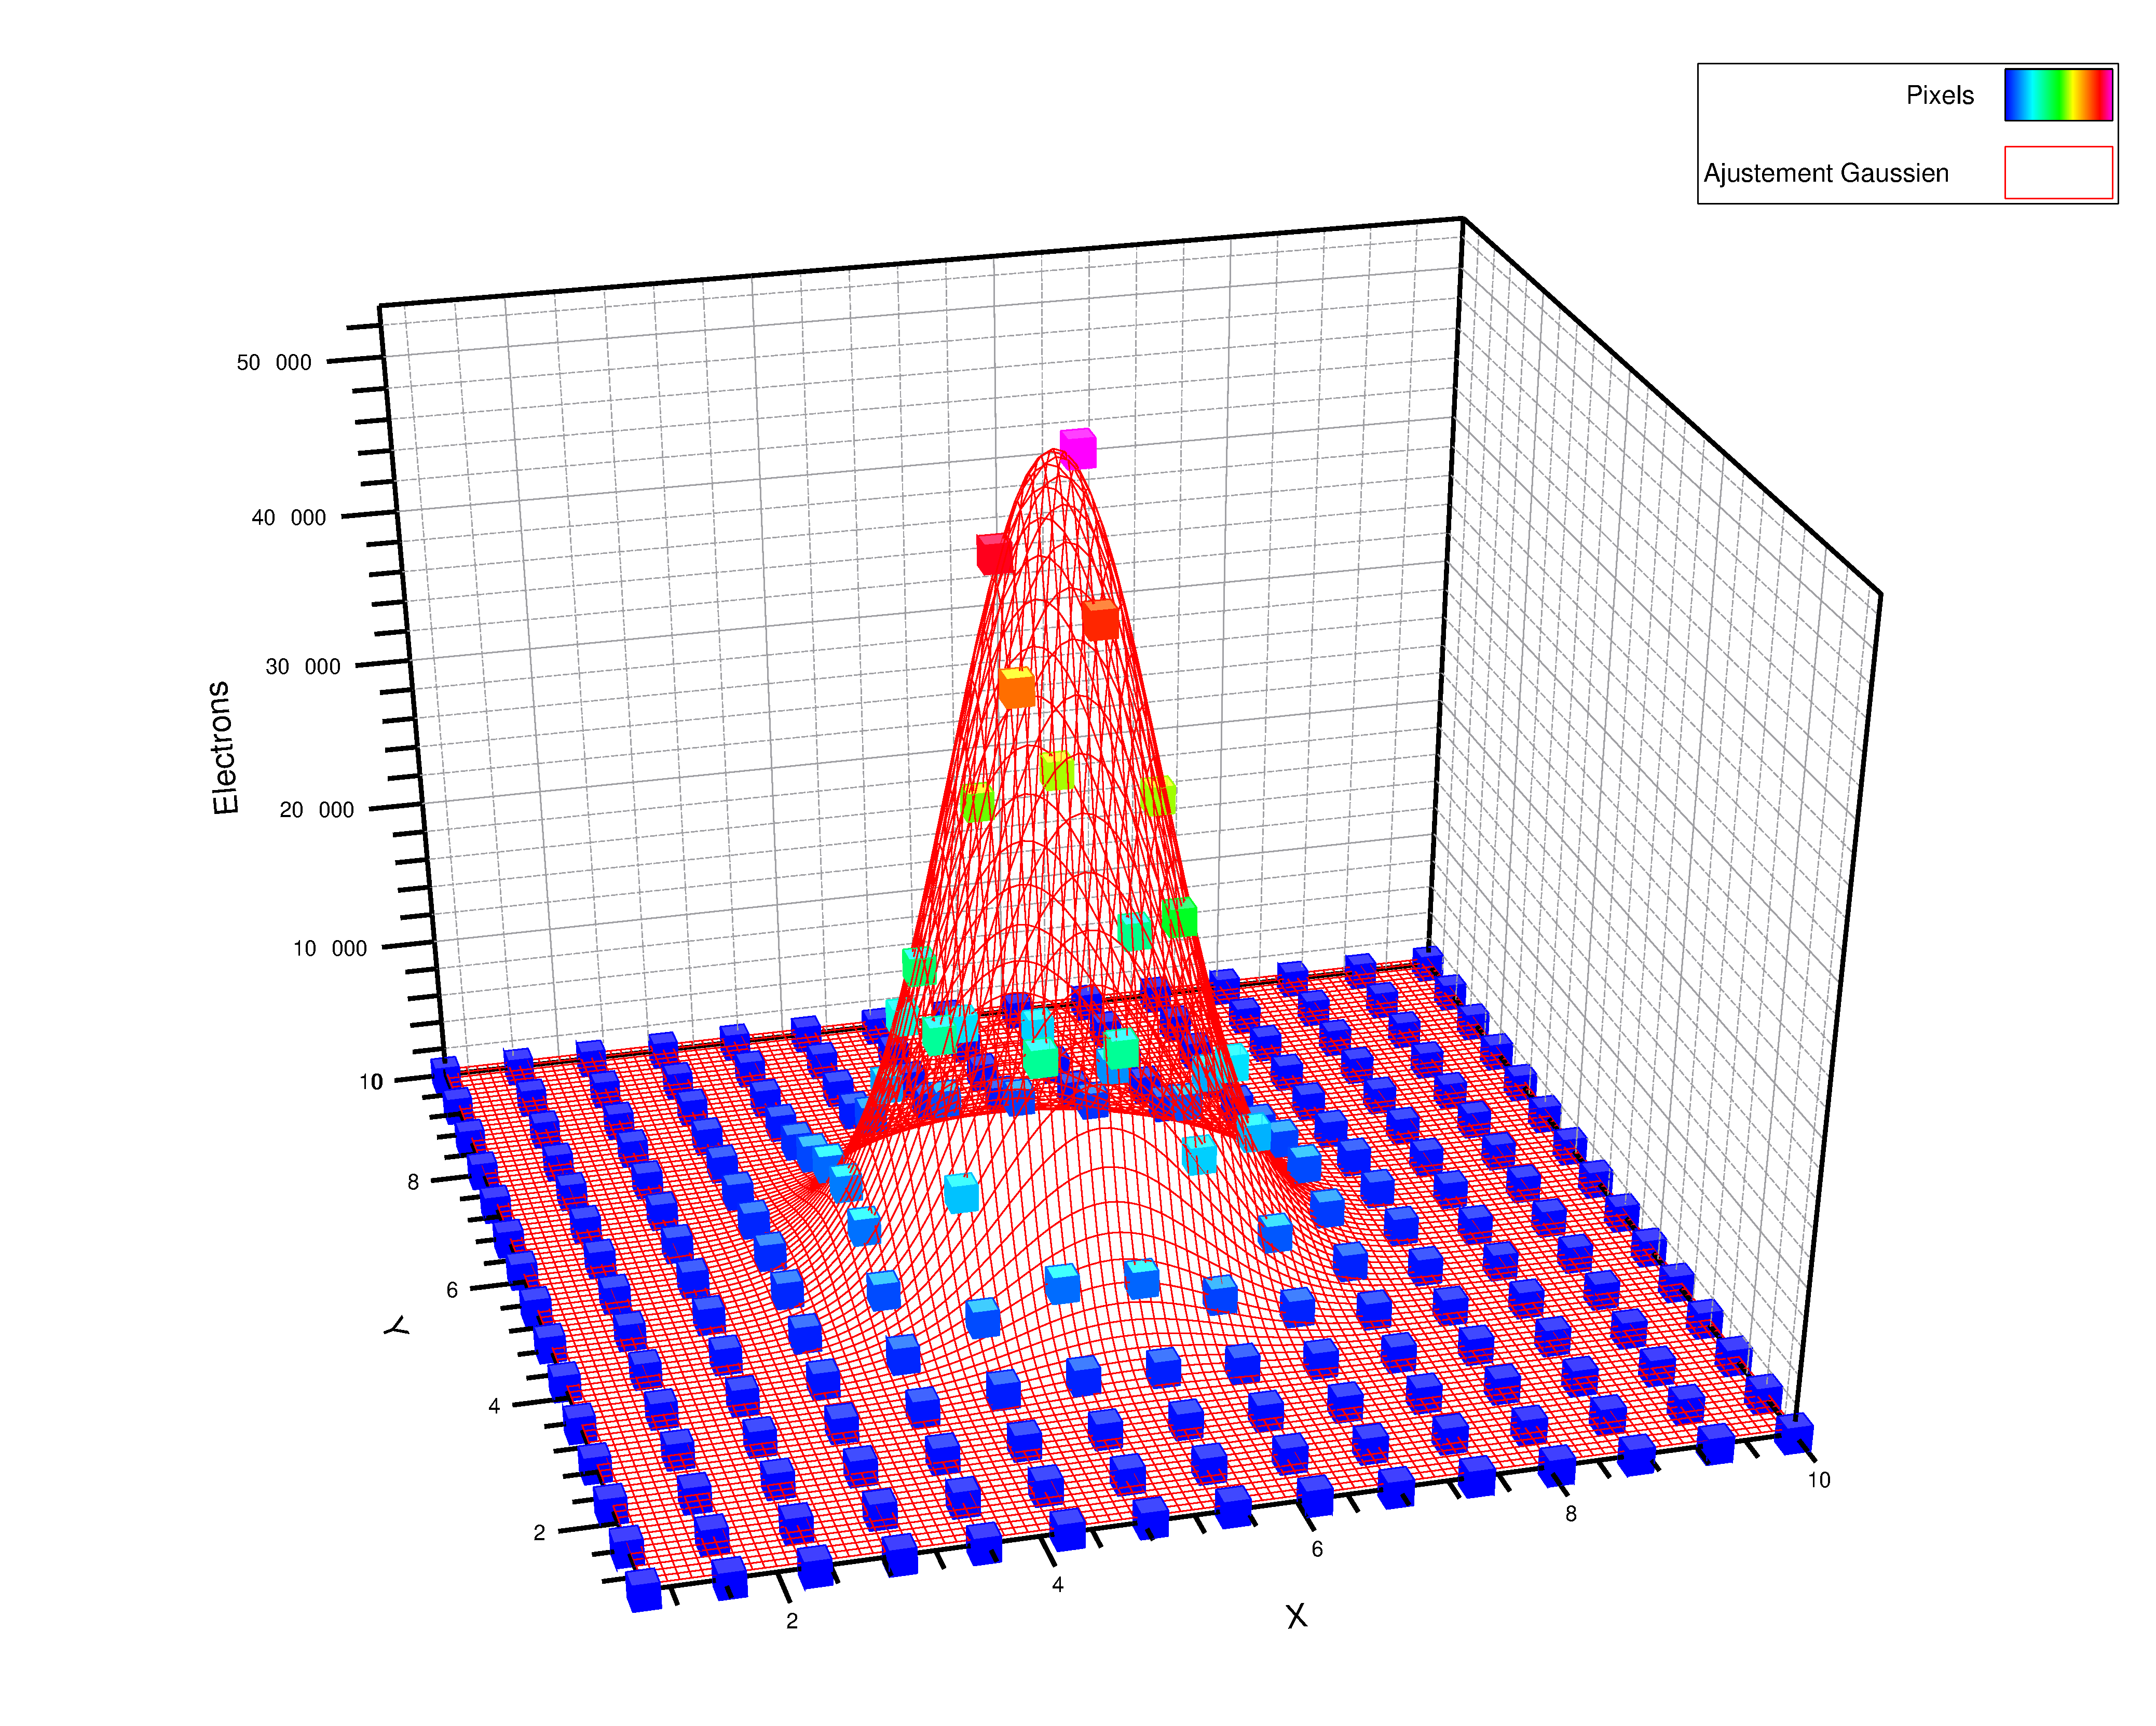
\includegraphics[width=0.6\linewidth]{fig/FWHM.pdf}
        \caption{Visualisation des photons mesurés pour une étoile avec un important rapport signal/bruit\label{fwhm}}
\end{figure}

\noindent En Figure \ref{fwhm} apparaît clairement que la source n'est effectivement pas parfaitement ponctuelle, et que le flux mesuré par le capteur est réparti sur plusieurs pixels. Nous avons également superposé un ajustement selon une Gaussienne en 3D, modèle le plus proche de nos valeurs, et permettant donc de justifier l'utilisation du terme de FWHM, que nous avons donc déterminé à partir de cette modélisation. Il est important de relever qu'à partir du moment où l'on considère une gausienne en 3D, la notion de FWHM dépend de la direction ($x$ ou $y$), le rapport entre ces deux FWHM définit même la rondeur $r$ de l'étoile (plus $r$ est proche de 1, plus l'étoile est dite ronde). Dans notre cas cependant, la rondeur est de $r=1.009$, nous allons donc pendant notre étude considérer nos sources comme parfaitement rondes et prendront la moyenne des deux FWHM comme paramètre de détection. Nous avons donc à partir des paramètres de modélisation déterminés par $Qtiplot$ obtenus une largeur à mi-hauteur de:

\[\boxed{\text{FWHM}=1.95 \; \text{pixels}}\]

\noindent Nous considérerons cette grandeur comme sans incertitude, celle-ci étant trop délicate à implémenter dans notre fonction de détection de sources, et de toute manière très faible grâce au choix d'une étoile avec un important rapport signal/bruit (on s'attend à ce que son profil soit le plus proche possible de la PSF de notre acquisition). \\

Le prochain paramètre que nous allons aborder est celui du pic maximum. Celui-ci est relié au profil de nos sources que nous venons de décrire, le pixel qui va détecter le point central de la PSF va donc mesurer la plus grande valeur en électrons (dans le cas idéal ou ce point est centré sur un pixel, il peut également tomber entre plusieurs pixels et dans ce cas on observera plusieurs pixels qui auront des valeurs proches du pic). Cette valeur de pic nous permet donc de définir un critère de sélection des sources, car nous cherchons à éviter de travailler avec des sources qui auraient saturé le capteur, car nous perdrions de l'information et cela mènerait à des mesures fausses. Nous voyons sur la Table \ref{CCD} que la capacité maximale de notre capteur est de $10 ^{5} e-$, soit environ $65000$ ADU. Nous avons choisi de définir ce critère de saturation à $50 000$ ADU, car nous avons très peu de sources au-delà de cette valeur, nous en excluons donc une faible quantité tout en étant ainsi sûr d'être suffisamment loin du niveau de saturation du capteur. Le gain permettant de convertir les électrons mesurés en ADU, nous posons finalement le pic maximum comme:

\[\boxed{\text{Pic Maximum} = \text{Gain}*50 000 \; \text{électrons}}\]

Finalement, le dernier critère de détection que nous devons considérer est celui du "seuil" ("treshold" en anglais), soit la valeur à partir de laquelle un pixel sera considéré comme une source. Celle-ci est généralement exprimée comme un multiple de la valeur du fond de ciel, sur lequel nous allons revenir plus en détail, mais qui correspond à la valeur mesurée par le CCD en dehors des sources elles-même. Une valeur trop proche de celle du fond de ciel signifie que l'on considérera par erreur des pixels chauds ou de simples variations du fond comme des sources, tandis qu'une valeur trop haute implique que nous considérerons simplement moins d'étoiles, ce paramètre peut donc dans notre cas être utilisé pour sélectionner plus ou moins d'étoiles, en considérant que nous plus ce paramètre baisse, plus les nouvelles étoiles détéctées auront un flux faible, ainsi on s'attend à globalement ajouter des étoiles avec un moins bon rapport signal bruit en baissant le seuil. En jouant sur ce paramètre, nous avons choisi un paramètre arbitrairement, nous permettant de détecter un nombre de source suffisant pour effectuer une bonne calibration sans avoir de risque de détecter de "faux positifs":

\[\boxed{\text{Seuil}=\text{Fond de ciel}*100 \; \text{électrons}}\]

\subsection{Méthodes d'annulation du fond de ciel\label{méthodes fond}}%
Maintenant que nous avons établis les paramètres avec lesquels nous détectons nos sources, discutons de la méthode que nous allons utiliser pour déterminer la valeur du fond de ciel de notre image. Nous avons à notre disposition deux méthodes, une détermination globale et une locale. Comme leur nom l'indique, la méthode globale sera de regarder le fond à l'échelle de toute notre image, tandis que la méthode locale regardera le fond de ciel au voisinage de chacunes de nos sources. Dans ces deux cas, nous nous intéresserons à la médiane des données que nous allons observer, car celle-ci sera plus robuste que la moyenne aux variations induites par les forts pics d'intensité des sources, ceux-ci étant concentrés sur une quantité limité de pixels à l'échelle de notre image, la médiane est une quantité statistique très proche de la valeur du fond de ciel. C'est une notion importante quand dans la suite de ce chapitre, nous allons nous intéresser à la notion de rayon d'ouverture optimal des sources pour la photométrie, et il est important de considérer que le flux reçu par le capteur correspondra à la somme des photons émis par les sources et ceux du fond de ciel, ainsi il sera important de corriger le flux de l'étoile par la valeur du fond de ciel sur l'aire considérée lorsque nous étudierons le rayon d'ouverture de nos étoiles. Regardons l'impact de chacunes de ces méthodes sur la correction du flux reçu en fonction de ce rayon:



\begin{figure}[h]
     \centering
     \begin{subfigure}[b]{0.49\textwidth}
         \centering
         \includegraphics[width=1\textwidth]{fig/bg corr.pdf}
         \caption{Correction du flux reçu pour une source quelconque en fonction de la méthode utilisée}
         \label{subfig:bgcorr}
     \end{subfigure}
    \hfill
         \begin{subfigure}[b]{0.445\textwidth}
             \centering
             \includegraphics[width=1\textwidth]{fig/local global.pdf}
             \caption{Valeur du fond de ciel calculée par la méthode globale et locale pour chaque sources détectées}
             \label{subfig:localglobal}
         \end{subfigure} 
      \caption{Confrontation des deux méthodes d'annulation du fond de ciel}
       \label{fig:localglobal}
\end{figure}

\noindent Lorsque nous parlerons de rayon d'ouverture, nous parlerons à chaque fois du rayon du masque de l'étoile, cependant la méthode d'annulation loale nécessite de définir un rayon intérieur et extérieur pour le masque appliqué autour de chaque sources. Pour déterminer ce dernier, nous avons dans un premier temps corrigé le flux du fond de ciel globalement comme on peut le voir en Figure \ref{subfig:bgcorr}, puis à partir de cela nous avons déterminé qu'au delà d'un rayon d'ouverture d'environ trois pixels, nous ne semblions plus recevoir de flux des sources en elle-même, et ce quelque soit la source considérée (nous pouvons observer pour cela le flux corrigé pour des étoiles différentes et observer que le profil est constant à travers les sources, comme en Figure \ref{annexe flux}). Ainsi, nous avons prit de manière relativement arbitraire un masque de rayons $r _{int}=4\text{pix}$ et $r _{ext}=6 \text{pix}$ pour le fond de ciel autour de nos sources. L'idée est d'avoir un échantillon suffisamment grand afin que les statistiques sur celui-ci soient pertinente, tandis qu'un masque trop grand augmente les chances de capter une autre source et non pas seulement le fond de ciel.
\noindent Pour finir sur l'annulation du fond de ciel, nous pouvons comparer la valeur de fond produite par ces deux méthodes pour chaque sources que nous avons détéctée, ce qui est visible en Figure \ref{fig:localglobal}, où nous constatons que la valeur estimée localement oscille autour de la valeur globale, sauf pour certaines sources où celui-ci est clairement sur-évalué, ce qui correspond donc au cas décrit précédemment où une autre source a été prise en compte par le masque de ciel. Nous sources étant triées par valeur d'intensité maximale de pic, nous constatons également que pour les étoiels avec les pics les plus importants, la valeur du fond de ciel semble drastiquement augmenter. Dans la suite de nos discussion sur les paramètres de calibration, nous utiliserons une méthode de calibration globale, puis nous comparerons l'impact de ces deux méthodes sur la calibration photométrique. 


\subsection{Rayon d'ouverture optimal}

 Nous l'avons rapidement abordé, le rayon d'ouverture est le paramètre le plus important à déterminer pour des mesures de photométrie d'ouverture, car celui-ci a un impact sur le flux mesuré et donc la magnitude, mais également le rapport signal/bruit de notre source, il est ainsi crucial de le fixer rigoureusement afin de calibrer avec précision notre zéro. En effet, pour exploiter les informations mesurées par le capteur CCD provenant d'une source, il faut appliquer un masque circulaire autour de celle-ci, d'un rayon le rayon d'ouverture. Traditionnelement, ce rayon est exprimé comme un multiple de la FWHM, car il peut se déterminer selon la PSF de notre image, or dans notre cas nous utiliserons des méthodes "expérimentales" pour le fixer, cela a donc moins de sens, car nous balayerons toutes les valeurs possibles quoiqu'il arrive. Nous avons donc choisi de conserver cette convention de $R=r*FWHM$ avec $R$ le rayon d'ouverture et $r$ le facteur sur la FWHM et ainsi lorsque nous parlerons de rayons d'ouverture dans la suite du rapport nous parlerons de $r$. 
\subsubsection{Notion de rapport signal/bruit\label{Label}}%
Avant de présenter les différentes méthodes que nous avons utilisées pour déterminer ce rayon d'ouverture, introduisons rapidement la notion de rapport signal/bruit. En effet, de par son fonctionnement, un capteur CCD produit nécessairements des électrons dus à agitation thermique, au bruit de lecture, les imperfections des lentilles... Afin de quantifier ces électrons constituants le bruit de nos mesure nos introduisons donc la notion de rapport signal/bruit (RSB), qui quantifie la portion de notre mesure qui correspond réellement à des photons émis par les sources que nous observons. Il s'exprime comme:

\[\text{RSB}=\frac{N _{*}}{\sqrt{N _{*}+n _{pix}(N _{S}+N _{D} + N _{R}^2)}}\]

\noindent Avec $N _{*}$ le flux mesuré sur la source, $n _{pix}$ le nombre de pixels utilisés pour la mesure, $N _{S}$ la valeur du fond de ciel, $N _{D}$ le bruit d'obscurité (le courant d'obscurité multiplié par le temps d'exposition) et enfin $N _{R}$ le bruit de lecture. Ces informations seront tirés des tables \textbf{REFERENCE A AJOUTER} 
\subsubsection{Critère RSB sur chaque étoile\label{Label}}%
Maintenant que nous avons introdtui la notion de RSB, nous allons pouvoir décrire les trois méthodes dont nous allons discuter pour déterminer le rayon d'ouverture optimal, à commencer par un critère simple: étant donné que plus le RSB est élevé plus l'information mesurée provient effectivement de la source étudiée, nous allons chercher à faire varier le rayon d'ouverture pour chaque étoile détectée et cherche la valeur pour laquelle le RSB est maximal, ainsi nous travaillerons avec le signal le plus propre possible.

\begin{figure}[h]
        \centering
        \includegraphics[width=0.5\linewidth]{fig/snr all.pdf}
        \caption{Rapport signal/bruit en fonction du rayon d'ouverture pour différentes étoiles}
        \label{rsb all}
\end{figure}

\noindent Comme nous pouvons nous y attendre à partir de son expression, nous constatons en Figure \ref{rsb all} que tant que le rayon d'ouverture est assez faible, l'augmenter revient à considérer davantages de photons provenant de la sources, tandis qu'au-delà d'un certaine valeur (proche de la valeur dont nous discutions du flux), nous ne recevons plus que des photons du fond de ciel ce qui considérant la correction que nous avons effectuée revient donc à augmenter le bruit. Le rayon optimal, bien que semblant varier assez faiblement, n'est pas le même pour toutes les sources que nous considérons, ainsi il semble pertinent d'établir un rayon optimal pour chaque étoile, et nous reviendrons sur cette pertinence lorsque nous étudierons l'impact de ce choix sur la précision de la calibration. 
\subsubsection{Critère du RSB le plus faible\label{Label}}%
Un autre raisonnement que nous pouvons établir pour déterminer le rayon d'ouverture optimal est le suivant: étant donné que nous pouvons faire l'approximation que le RSB augmente avec le valeur de pic (cela n'est pas linéaire, cependant sur le nombre de sources avec lequel nous travaillons et les variations de RSB en jeu, c'est une approximation suffisante), nous pouvons alors chercher à trouver le rayon optimal d'une étoile avec une faible valeur de pic et utiliser cette valeur pour toutes nous sources. L'idée est que si l'on cherche à avoir un critère fixe sur chaque étoiles, cette méthode permet de s'assurer que nous regardons le scénario où les variations relative (à sa valeur maximum) du RSB sont les plus importantes, transposer ce rayon aux autres étoiles aura donc moins d'impact sur leur RSB que si nous utilisions un critère sur l'étoile avec le meilleur RSB.

\subsubsection{Méthode d'optimisation Flux-RSB\label{fluxrsb}}%

Finalement, la dernière méthode que nous avons considérée pour fixer le rayon optimal d'ouverture est une méthode cherchant à trouver le point optimal en prenant en compte à la fois RSB et flux. L'idée est que si l'on normalise le flux et le RSB, nous pourrons établir un critère sur les deux paramètres, car si l'on considère uniquement le RSB, on constate que la quantité de flux correspondant au rayon optimal n'est pas la valeur asymptotique, une partie des photons provenant de l'étoile n'est donc pas considérée, ainsi l'idée est de trouver le point maximisant le RSB le plus proche de la valeur maximale du flux corrigé, ce qui n'a du sens que si l'on considère ces deux grandeurs normalisées.

\begin{figure}[h]
        \centering
        \includegraphics[width=0.5\linewidth]{fig/snr-flux.pdf}
        \caption{RSB et flux en fonction du rayon d'ouverture pour une source quelconque}
        \label{gsnrflux}
\end{figure}

\noindent Cette méthode, tout comme la dernière, est donc une méthode déterminant un rayon optimal pour chaque source. Elle est d'autant moins robuste face aux sources qui seraient très proches les unes de autres comme dans le cas d'étoiles binaires car on commence très vite à recevoir des photons de la seconde étoile et cela "casse" la normalisation, le rayon produit n'est donc pas pertinent dans certains cas, et maintenant que nous avons décrit les différentes méthodes que nous avons considérés pour déterminer les paramètres importants à la calibration, regardons l'impact de ces derniers sur la précision avec laquelle nous arrivons à fixer le zéro de notre magnitude instrumentale. 
\subsection{Impact de chaque méthodes sur la calibration\label{Label}}%
  Commençons rapidement par préciser qu'afin de fixer notre constante de zéro B, nous devons avoir accès aux magnitudes de références de toutes les sources que nous consisdérons. Dans notre cas, le nombre de sources est d'environ 300, il est donc important de trouver le moyen d'automatiser la récolte des magnitudes référencées. Pour cela, nous commençons par utiliser l'outil \textit{Nova Astrometry}, qui permet grâce à une large base de données d'images du ciel de traduire les positions en pixels des sources de nos images en positions exprimées en coordonées célestes. Ainsi, une fois cette conversion effectuée, nous pouvons interroger le catalogue \textit{UCAC4} \textbf{REFERENCE A AJOUTER} pour obtenir les magnitudes de référence pour le fitre considéré. \\

  \noindent Finalement, nous calculons la constante $B$ associée, pour chaque source et moyennons l'ensemble des valeurs obtenues pour obtenir notre zéro à l'écart-type près. Nous pouvons ainsi maintenant regarder l'impact qu'ont les différentes méthodes de détermination du rayon optimal d'ouverture sur l'incertitude associée à la calibration du zéro, et ce pour un même jeu d'étoiles.

\begin{figure}[h]
     \centering
     \begin{subfigure}[b]{0.49\textwidth}
         \centering
         \includegraphics[width=1\textwidth]{fig/incert.pdf}
         \caption{Incertitude sur B en fonction du nombre d'étoiles utilisées pour effectuer la calibration}
         \label{subfig:incert}
     \end{subfigure}
     \hfill
          \begin{subfigure}[b]{0.49\textwidth}
              \centering
              \includegraphics[width=1\textwidth]{fig/incert corr.pdf}
              \caption{Incertitude sur B en fonction du nombre d'étoiles utilisées pour effectuer la calibration (après correction)}
              \label{subfig:incert corr}
          \end{subfigure}
          
      \caption{Impact des trois méthodes de détermination du rayon d'ouverture sur la précision du zéro}
       \label{fig:incert}
\end{figure}

En Figure \ref{fig:incert}, les sources sont triées par valeur de pic décroissante, toujours en approximant cela veut dire que l'on considère globalement les étoiles avec le meilleur RSB en premier puis les moins bon rapports signal/bruit tandis que le nombre d'étoiles considérées augmente. Aussi, il est important de relever qu'en Figure \ref{subfig:incert}, on observe de forts pics d'augmentation de l'incertitude sur B, qui correspondent en réalités au scénario que l'on a déjà précédemment évoqué, notre méthode de calcul de la magnitude est très peu robuste dans le cas de sources trop proches, car nous n'avons pas de moyen de déterminer de quelle sources les photons mesurés proviennent. Afin d'éviter ces écarts, nous appliquons le critère de correction suivant: si l'ajout d'un étoile au jeu de calibration augmente l'incertitude de B au-delà de l'écart-type de l'ensemble des incertitudes, celle-ci est ignorée pour la calibration. Cela exclu environ une vingtaine d'étoiles, et mène à ce que l'on observe en Figure \ref{subfig:incert corr}, à partir de laquelle nous fixerons la valeur finale du zéro, à partir donc du nombre d'étoiles utilisé pour la calibration minimisant l'erreur sur ce dernier. Pour se convaincre que ce critère n'exclut pas simplement des étoiles qui traduirait une autre erreur dans notre méthode, observons ce qui a été mesuré par le capteur sur trois d'entre elles:

\begin{figure}[h]
     \centering
     \begin{subfigure}[b]{0.33\textwidth}
         \centering
         \includegraphics[width=1\textwidth]{fig/etoile ignorée red1.pdf}
         \caption{Première étoile exclue}
         \label{subfig:excl1}
     \end{subfigure}
     \hfill
          \begin{subfigure}[b]{0.33\textwidth}
              \centering
              \includegraphics[width=1\textwidth]{fig/etoile ignorée red2.pdf}
              \caption{Seconde étoile exclue}
              \label{subfig:excl2}
          \end{subfigure}
      \hfill
           \begin{subfigure}[b]{0.33\textwidth}
               \centering
               \includegraphics[width=1\textwidth]{fig/etoile ignorée red3.pdf}
               \caption{Troisième étoile exclue}
               \label{subfig:exlc3}
           \end{subfigure}
           
      \caption{Photons mesurés par le CCD pour trois étoiles écartées de la calibration}
       \label{fig:}
\end{figure}

Les Figures \ref{subfig:excl1} et \ref{subfig:excl2} confortent notre hypothèse: lorsque plusieurs sources sont trop proches, les magnitudes que nous calculons sont erronées car nous n'avons pas de méthode différente de calcul du rayon optimal et du flux pour ces dernières. La Figure \ref{subfig:exlc3} cependantmet en lumière un autre scénario que nous n'avions pas considéré: une étoile dont le flux n'est pas sur le champ d'observation du CCD, ainsi la magnitude que nous calculons n'est déduite que d'une fraction du flux de l'étoile, menant à un facteur de calibration erroné.\\

Nous pouvons enfin discuter de la méthode que nous allons retenir pour le rayon d'ouverture optimal. La Figure \ref{subfig:incert corr} nous permet assez facilement d'établir que le critère permettant la calibration la plus précise est celui du critère RSB sur l'étoile avec le pic le plus faible en effet la PSF étant censée être constante à travers notre image ,l'étalement des sources est également constant, ainsi fixer le rayon de cette manière permet d'obtenir un RSB maximal sur toutes les sources sans changer le rayon d'ouverture. Malgré ce dont nous discutions en Section \ref{fluxrsb}, le fait de ne pas mesurer l'entièreté du flux de l'étoile n'est pas un problème dans que la fraction mesurée est la même pour chaque source, la constante B va donc absorber l'écart que cela induit.\\

Enfin, nous allons observer l'impact des deux méthodes d'annulation du fond de ciel dont nous discutions en Section \ref{méthodes fond} sur l'incertitude de notre zéro de magnitiude, afin de déterminer la mathode optimale. Pour cela, regardons la valeur optimale (fixée à partir de la Figure \ref{subfig:incert corr}) de B pour chaque méthode:

\begin{table}[H]
    \centering
    \begin{tabular}{c|c|c}
         & Fond de ciel global & Fond de ciel local \\
        \hline
        Critère RSB sur chaque source & $23.892 \pm 0.096$ & $23.892 \pm 0.096$ \\
        \hline
        Optimisation RSB/Flux& $23.946 \pm 0.064$ & $23.936 \pm 0.065$\\
        \hline
         Critère RSB sur l'étoile avec le pic le plus faible & $23.828 \pm 0.062$ & $23.828 \pm 0.062$ \\
     \end{tabular}
    \caption{Constante B en fonction des critères utilisés pour fixer les paramètres photométriques (mag)}
    \label{mag}
\end{table}

\noindent Nous pouvons constatons sur la Table \ref{mag} que les variations que nous observions en Figure \ref{subfig:localglobal} n'étaient pas signiticatives aux échelles de flux que nous considérons ici, ainsi, car elles produisent une incertitude supérieure ou égale sur la constante de calibration aussi nous retiendrons la méthode globale car si celle-ci ne produit pas d'erreur supplémentaire elle reste la plus efficace.

\subsection{Calibration finale\label{cal}}%
  Nous avons désormais déterminé que les paramètres produisant la calibration la plus précise sont une annulation globale de la valeur du fond de ciel avec un rayon d'ouverture fixé par la méthode du RSB de l'étoile au plus faible pic. Nous retiendrons finalement les valeurs suivantes pour le zéro de magnitude pour les filtres r et g, en transposant le raisonnement que l'on vient d'exposer au second filtre. Finalement, nous obtenons:

  \begin{align*}
    &\boxed{B _{r}=23.946 \pm 0.062 \; \text{mag}} &\boxed{B _{g}=23.85 \pm 0.084 \; \text{mag}}
  \end{align*}
  
\noindent L'incertitude que nous obtenons pour le second filtre étant plus élevée car à seuil de détection égal, nous détectons moins de sources, or diminuer ce seuil augmente les chances de détecter de "faux positifs" et ajoute des source de faible RSB, cela n'augmente donc pas la précision sur la calibration. 
  
\section{Mesures photométriques et incertitudes}
Mainteant que la calibration photométrique a été effectuée sur nos deux images, nous pouvons procéder à des mesures de magnitudes sur des étoiles en dehors du jeu de données utiilisé pour la calibration. Etant donné que nous avons cherché à maximiser le nombre de sources utilisées pour la calibration afin d'en maximiser la précision, nous allons diminuer légèrement le seuil de détection afin de détecter une vingtaine d'étoiles supplémentaires mais dont le RSB ne sera pas aussi optimal que ceux des étoiles du jeu de calibration. Calculons alors leur magnitude à l'incertitude de calibration près et confrontons les aux valeurs de références:

\begin{figure}[h]
     \centering
     \begin{subfigure}[b]{0.45\textwidth}
         \centering
         \includegraphics[width=1\textwidth]{fig/final r.pdf}
         \caption{Magnitudes calculées pours des étoiles (RSB $\approx$ 30) en dehors du jeu de calibration (filtre r)}
         \label{subfig:oui}
     \end{subfigure}
     \hfill
          \begin{subfigure}[b]{0.45\textwidth}
              \centering
              \includegraphics[width=1\textwidth]{fig/final g.pdf}
              \caption{Magnitudes calculées pours des étoiles (RSB $\approx$ 30) en dehors du jeu de calibration (filtre g)}
              \label{subfig:oui2}
          \end{subfigure} 
      \caption{Mesures de magnitudes sur de nouvelles sources après calibration photométrique}
       \label{fig:final}
\end{figure}


\noindent Aux incertitudes de calibration près, nous semblons obtenir des magnitudes pertinentes pour la plupart de nos sources en Figure \ref{fig:final}, sauf pour certaines source dont les résultats semblent très loins des valeurs de référence et cela est encore une fois lié à la faible robustesse de notre méthode à des sources trop proches, si l'on regarde les données du capteur pour les points divergeants de la Figure \ref{subfig:oui} par exemple, nous confirmons cette hypothèse.
\vspace{10\baselineskip}

 \begin{figure}[h]
     \centering
     \begin{subfigure}[b]{0.33\textwidth}
         \centering
         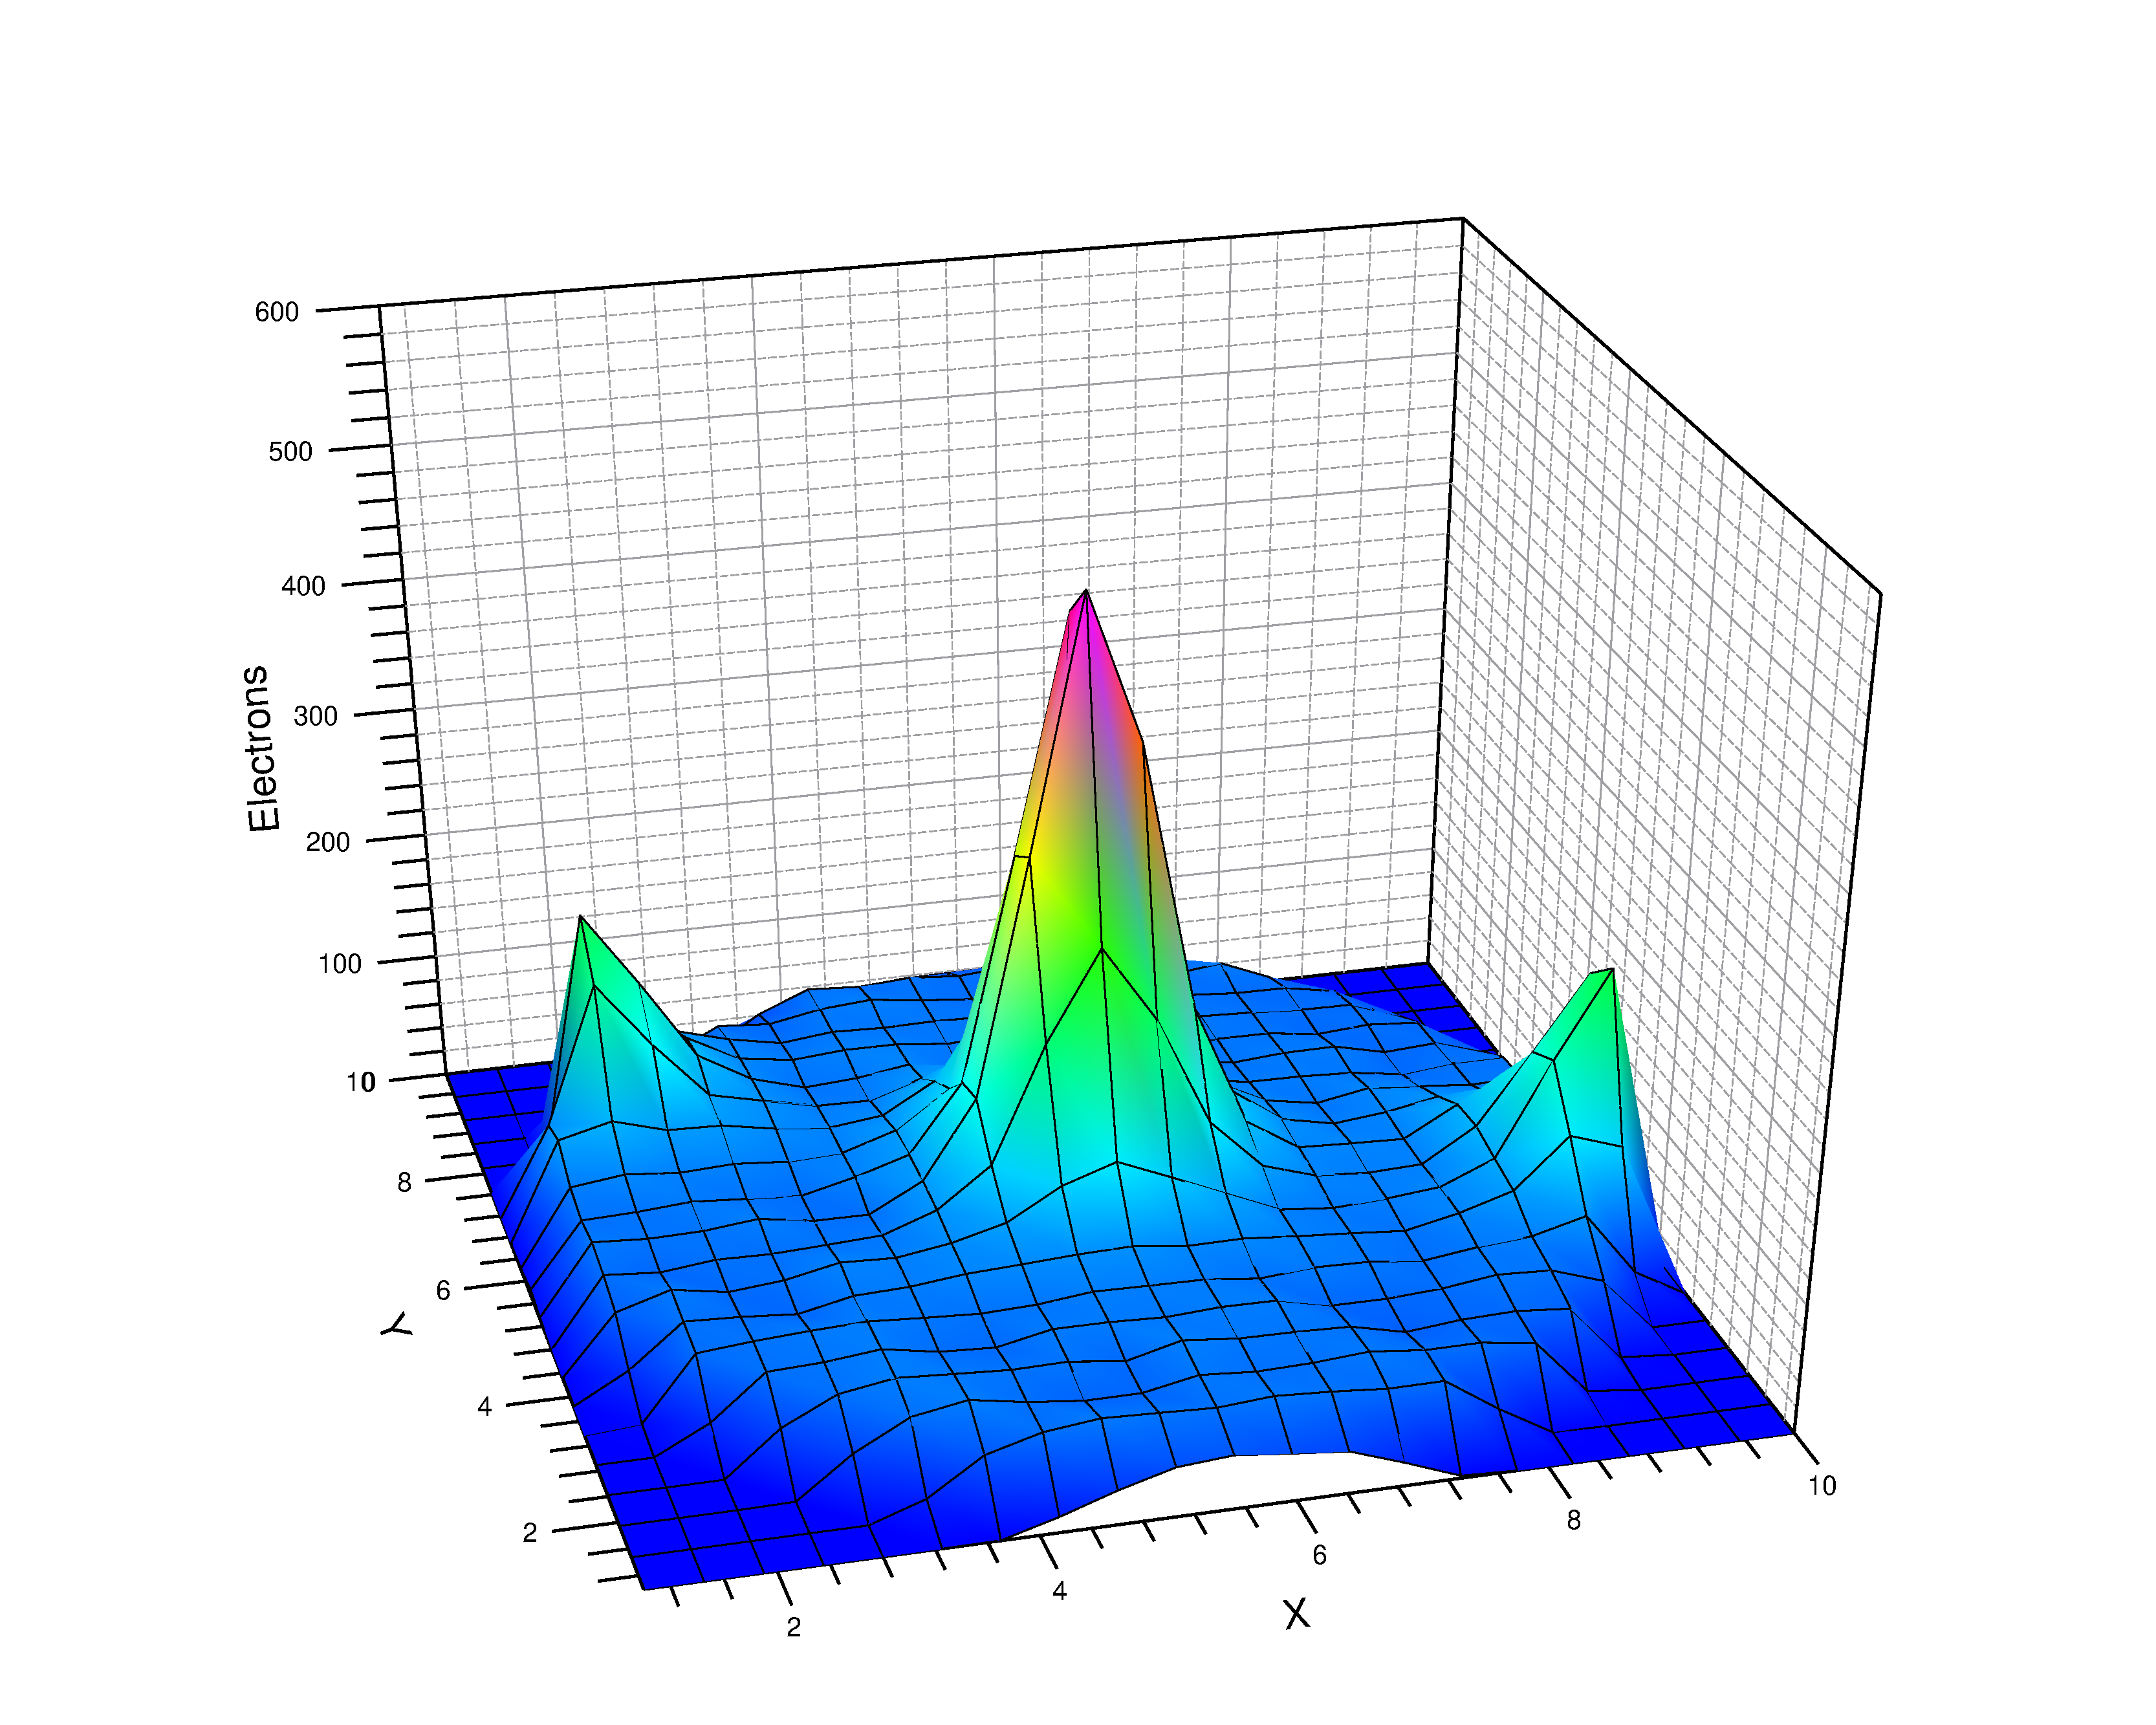
\includegraphics[width=1\textwidth]{fig/etoile divergente red1.pdf}
         \caption{Première étoile exclue}
         \label{subfig:excl1}
     \end{subfigure}
     \hfill
          \begin{subfigure}[b]{0.33\textwidth}
              \centering
              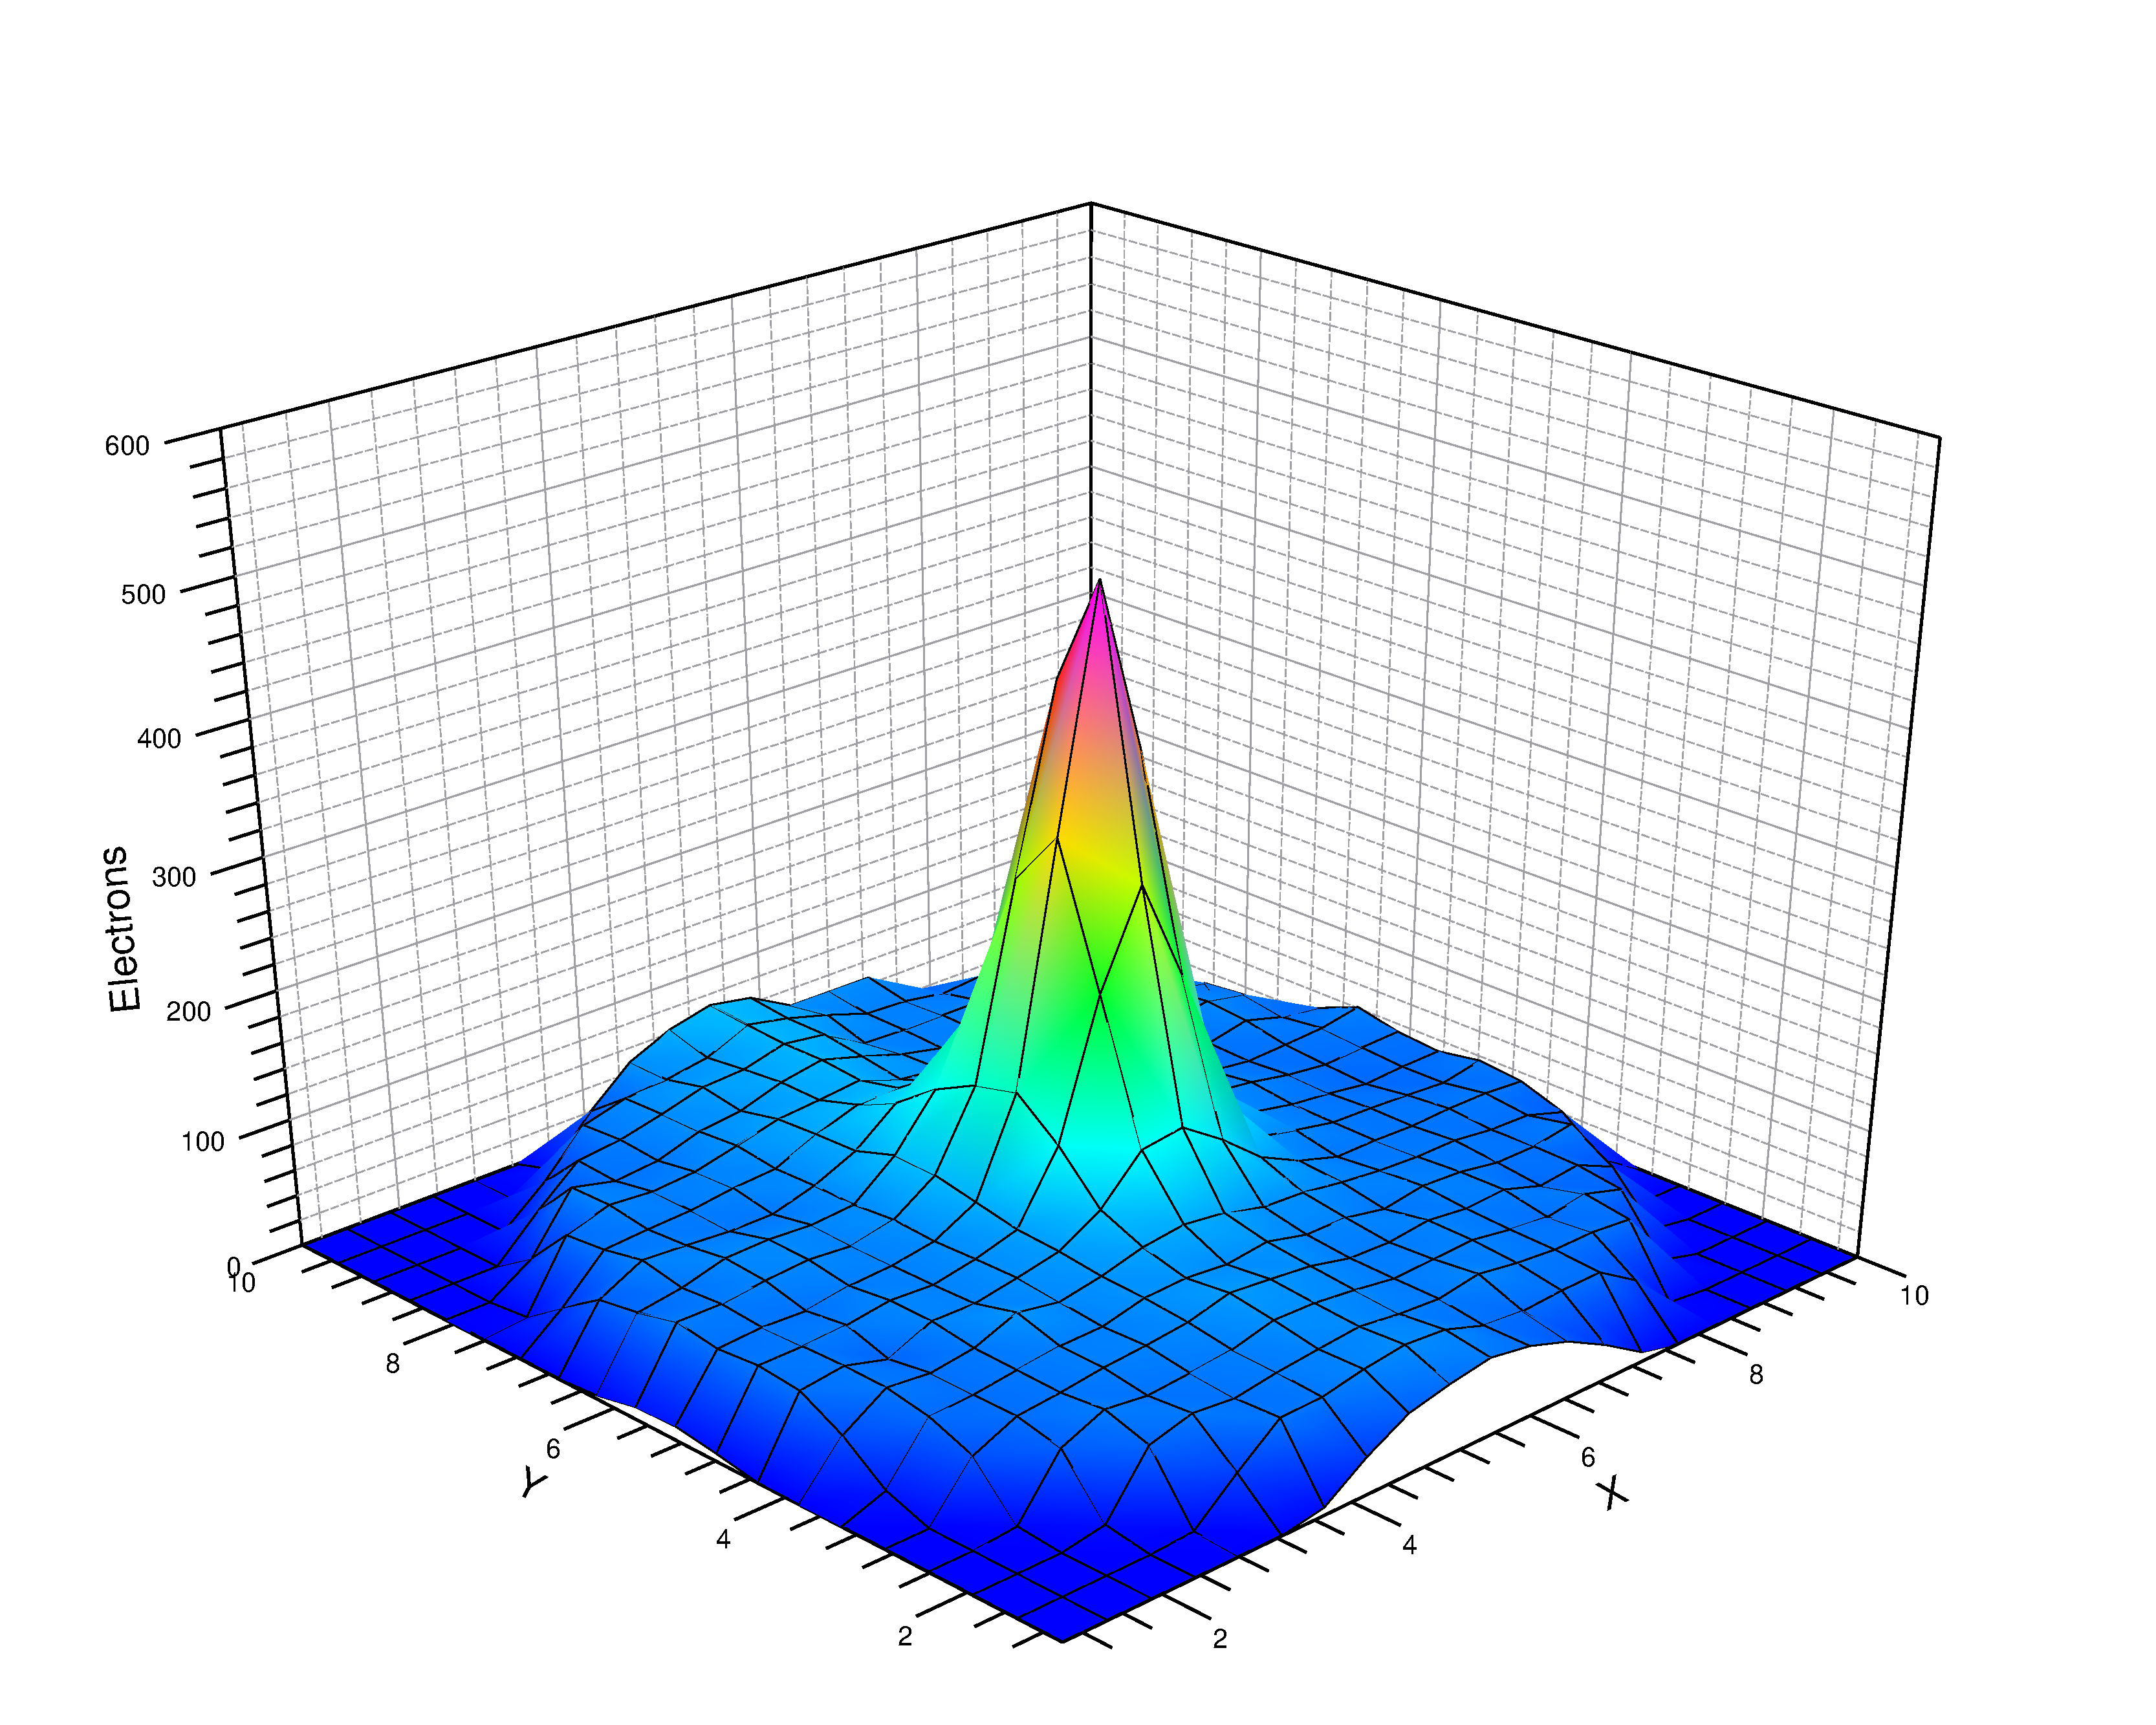
\includegraphics[width=1\textwidth]{fig/etoile divergente red2.pdf}
              \caption{Seconde étoile exclue}
              \label{subfig:excl2}
          \end{subfigure}
      \hfill
           \begin{subfigure}[b]{0.33\textwidth}
               \centering
               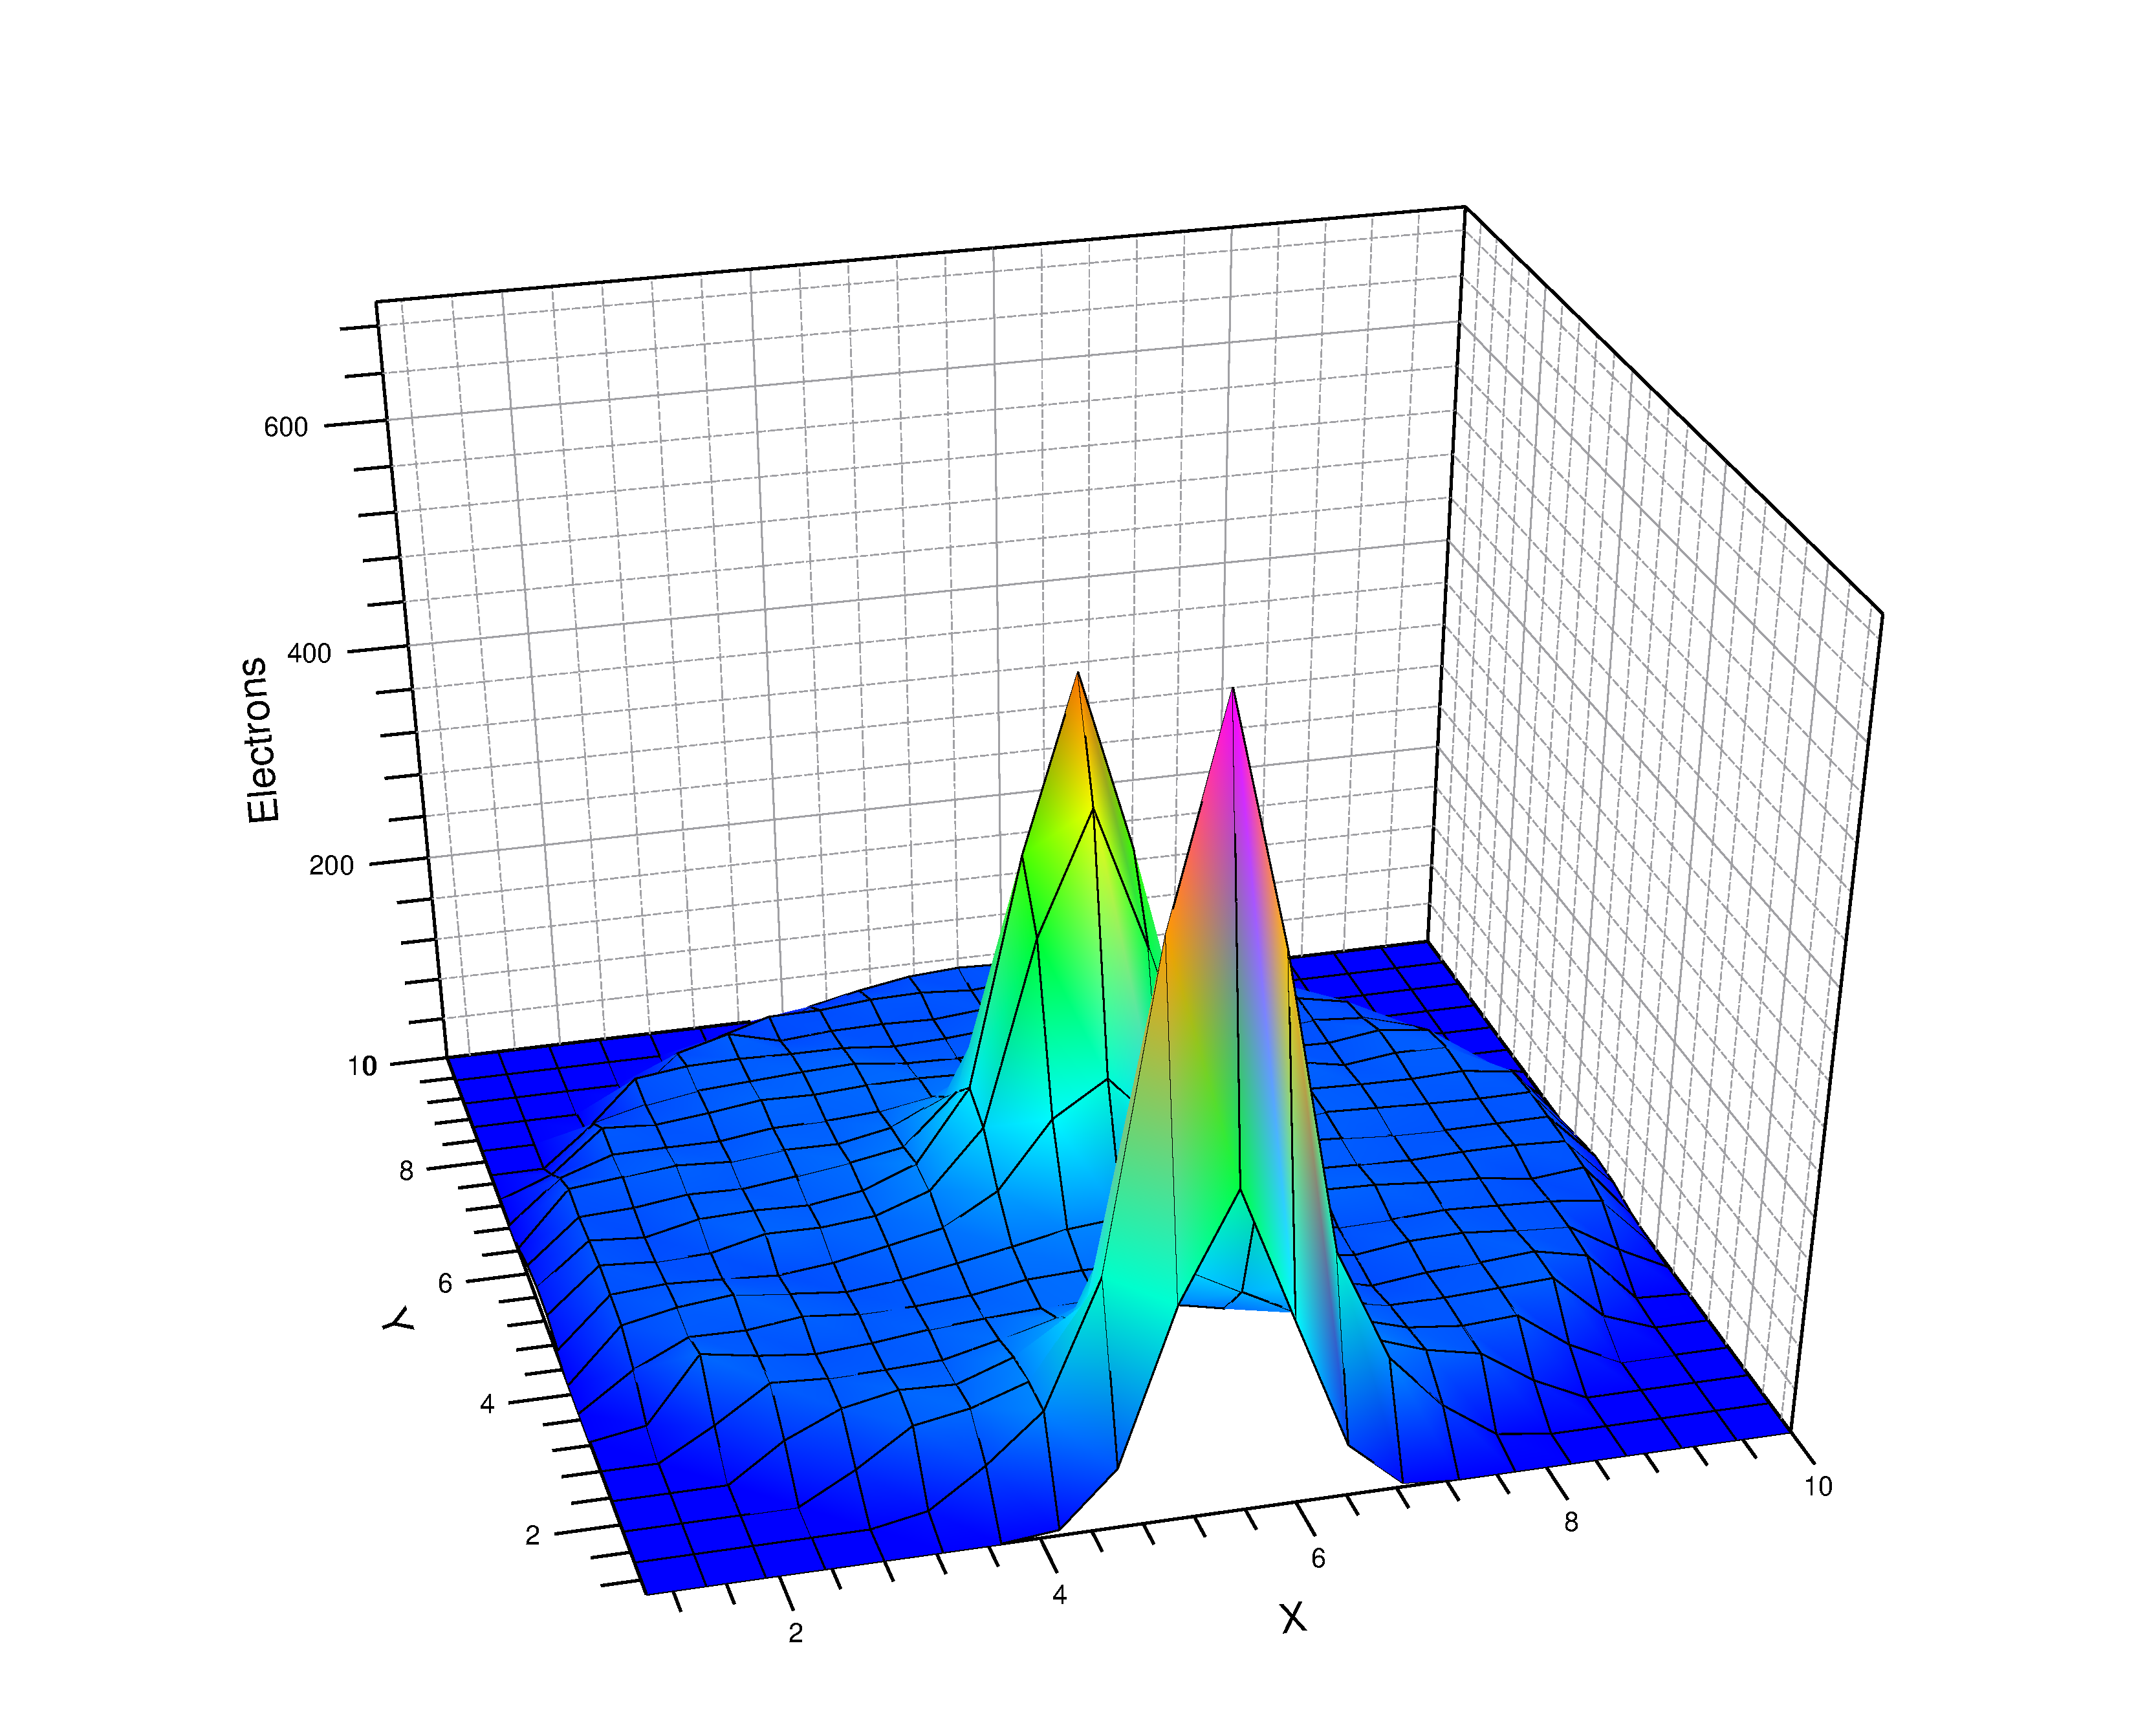
\includegraphics[width=1\textwidth]{fig/etoile divergente red3.pdf}
               \caption{Troisième étoile exclue}
               \label{subfig:exlc3}
           \end{subfigure}
           
      \caption{Photons mesurés par le CCD pour trois étoiles écartées de la calibration (filtre r)}
       \label{fig:exclu}
\end{figure} 

\noindent La Figure \ref{fig:exclu} nous montre encore une fois que dans le cas de sources trop proches les unes des autres, notre méthode de calcul de la magnitude ne produit plus de résultats pertinents.
% Pour les projets de spectroscopie : mesures de longueur d'onde, largeur équivalente, vitesse radiale, identification de raies spectrales
% Pour les projets de photométrie : mesure photométriques sur les étoiles cibles/références
